\documentclass[onesided]{article}\usepackage[]{graphicx}\usepackage[]{color}
% maxwidth is the original width if it is less than linewidth
% otherwise use linewidth (to make sure the graphics do not exceed the margin)
\makeatletter
\def\maxwidth{ %
  \ifdim\Gin@nat@width>\linewidth
    \linewidth
  \else
    \Gin@nat@width
  \fi
}
\makeatother

\definecolor{fgcolor}{rgb}{0.345, 0.345, 0.345}
\newcommand{\hlnum}[1]{\textcolor[rgb]{0.686,0.059,0.569}{#1}}%
\newcommand{\hlstr}[1]{\textcolor[rgb]{0.192,0.494,0.8}{#1}}%
\newcommand{\hlcom}[1]{\textcolor[rgb]{0.678,0.584,0.686}{\textit{#1}}}%
\newcommand{\hlopt}[1]{\textcolor[rgb]{0,0,0}{#1}}%
\newcommand{\hlstd}[1]{\textcolor[rgb]{0.345,0.345,0.345}{#1}}%
\newcommand{\hlkwa}[1]{\textcolor[rgb]{0.161,0.373,0.58}{\textbf{#1}}}%
\newcommand{\hlkwb}[1]{\textcolor[rgb]{0.69,0.353,0.396}{#1}}%
\newcommand{\hlkwc}[1]{\textcolor[rgb]{0.333,0.667,0.333}{#1}}%
\newcommand{\hlkwd}[1]{\textcolor[rgb]{0.737,0.353,0.396}{\textbf{#1}}}%
\let\hlipl\hlkwb

\usepackage{framed}
\makeatletter
\newenvironment{kframe}{%
 \def\at@end@of@kframe{}%
 \ifinner\ifhmode%
  \def\at@end@of@kframe{\end{minipage}}%
  \begin{minipage}{\columnwidth}%
 \fi\fi%
 \def\FrameCommand##1{\hskip\@totalleftmargin \hskip-\fboxsep
 \colorbox{shadecolor}{##1}\hskip-\fboxsep
     % There is no \\@totalrightmargin, so:
     \hskip-\linewidth \hskip-\@totalleftmargin \hskip\columnwidth}%
 \MakeFramed {\advance\hsize-\width
   \@totalleftmargin\z@ \linewidth\hsize
   \@setminipage}}%
 {\par\unskip\endMakeFramed%
 \at@end@of@kframe}
\makeatother

\definecolor{shadecolor}{rgb}{.97, .97, .97}
\definecolor{messagecolor}{rgb}{0, 0, 0}
\definecolor{warningcolor}{rgb}{1, 0, 1}
\definecolor{errorcolor}{rgb}{1, 0, 0}
\newenvironment{knitrout}{}{} % an empty environment to be redefined in TeX

\usepackage{alltt}
\usepackage[T1]{fontenc}
\linespread{1.5} % Line spacing - Palatino needs more space between lines
\usepackage{microtype} % Slightly tweak font spacing for aesthetics

\usepackage[hmarginratio=1:1,columnsep=20pt]{geometry} % Document margins
%\usepackage{multicol} % Used for the two-column layout of the document
\usepackage[hang, small,labelfont=bf,up,textfont=it,up]{caption} % Custom captions under/above floats in tables or figures
\usepackage{booktabs} % Horizontal rules in tables
\usepackage{float} % Required for tables and figures in the multi-column environment - they need to be placed in specific locations with the [H] (e.g. \begin{table}[H])

\usepackage{lettrine} % The lettrine is the first enlarged letter at the beginning of the text
\usepackage{paralist} % Used for the compactitem environment which makes bullet points with less space between them

% to ignore texts: good for thank messages and paper submissions.
      % \fbox{\phantom{This text will be invisible too, but a box will be printed arround it.}}

\usepackage{abstract} % Allows abstract customization
\renewcommand{\abstractnamefont}{\normalfont\bfseries} % Set the "Abstract" text to bold
%\renewcommand{\abstracttextfont}{\normalfont\small\itshape} % Set the abstract itself to small italic text

\usepackage[]{titlesec} % Allows customization of titles
\renewcommand\thesection{\Roman{section}} % Roman numerals for the sections
\renewcommand\thesubsection{\Roman{subsection}} % Roman numerals for subsections
\titleformat{\section}[block]{\large\scshape\centering}{\thesection.}{1em}{} % Change the look of the section titles
\titleformat{\subsection}[block]{\large}{\thesubsection.}{1em}{} % Change the look of the section titles

\usepackage{fancybox, fancyvrb, calc}
\usepackage[svgnames]{xcolor}
\usepackage{physics}
\usepackage{epigraph}
\usepackage{longtable}
\usepackage{pdflscape}
\usepackage{graphics}
\usepackage{pbox} % \pbox{20cm}{This is the first \\ cell}
\usepackage{amsfonts}
\usepackage{amsmath}
\usepackage{amssymb}
\usepackage{rotating}
\usepackage{paracol}
\usepackage{textcomp}
\usepackage[export]{adjustbox}
\usepackage{afterpage}
\usepackage{filecontents}
\usepackage{color}
\usepackage{latexsym}
\usepackage{lscape}       %\begin{landscape} and \end{landscape}
\usepackage{wasysym}
\usepackage{dashrule}
\usepackage{marvosym} % face package
\usepackage{framed}
\usepackage{tree-dvips}
\usepackage{pgffor}
\usepackage[]{authblk}
\usepackage{setspace}
\usepackage{array}
\usepackage[latin1]{inputenc}
\usepackage{hyperref}     %desactivar para link rojos
\usepackage{graphicx}
\usepackage{dcolumn} % for R tables
\usepackage{multirow} % For multirow in tables
\usepackage{pifont}
\usepackage{listings}
\usepackage{bm}




% hypothesis / theorem package begin
\usepackage{amsthm}
\usepackage{thmtools}
\declaretheoremstyle[
spaceabove=6pt, spacebelow=6pt,
headfont=\normalfont\bfseries,
notefont=\mdseries, notebraces={(}{)},
bodyfont=\normalfont,
postheadspace=0.6em,
headpunct=:
]{mystyle}
\declaretheorem[style=mystyle, name=Hypothesis, preheadhook={\renewcommand{\thehyp}{H\textsubscript{\arabic{hyp}}}}]{hyp}

\usepackage{cleveref}
\crefname{hyp}{hypothesis}{hypotheses}
\Crefname{hyp}{Hypothesis}{Hypotheses}
% hypothesis / theorem package end


%----------------------------------------------------------------------------------------
% Other ADDS-ON
%----------------------------------------------------------------------------------------

% independence symbol \independent
\newcommand\independent{\protect\mathpalette{\protect\independenT}{\perp}}
\def\independenT#1#2{\mathrel{\rlap{$#1#2$}\mkern2mu{#1#2}}}







\hypersetup{
    bookmarks=true,         % show bookmarks bar?
    unicode=false,          % non-Latin characters in Acrobat's bookmarks
    pdftoolbar=true,        % show Acrobat's toolbar?
    pdfmenubar=true,        % show Acrobat's menu?
    pdffitwindow=true,     % window fit to page when opened
    pdfstartview={FitH},    % fits the width of the page to the window
    pdftitle={My title},    % title
    pdfauthor={Author},     % author
    pdfsubject={Subject},   % subject of the document
    pdfcreator={Creator},   % creator of the document
    pdfproducer={Producer}, % producer of the document
    pdfkeywords={keyword1} {key2} {key3}, % list of keywords
    pdfnewwindow=true,      % links in new window
    colorlinks=true,       % false: boxed links; true: colored links
    linkcolor=ForestGreen,          % color of internal links (change box color with linkbordercolor)
    citecolor=ForestGreen,        % color of links to bibliography
    filecolor=ForestGreen,      % color of file links
    urlcolor=ForestGreen           % color of external links
}

%\usepackage[nodayofweek,level]{datetime} % to have date within text

\newcommand{\LETT}[3][]{\lettrine[lines=4,loversize=.2,#1]{\smash{#2}}{#3}} % letrine customization



% comments on margin
  % Select what to do with todonotes: 
  % \usepackage[disable]{todonotes} % notes not showed
  \usepackage[draft]{todonotes}   % notes showed
  % usage: \todo{This is a note at margin}

\usepackage{cooltooltips}

%%% bib begin
\usepackage[american]{babel}
\usepackage{csquotes}
\usepackage[backend=biber,style=authoryear,dashed=false,doi=false,isbn=false,url=false,arxiv=false]{biblatex}
%\DeclareLanguageMapping{american}{american-apa}
\addbibresource{/Users/hectorbahamonde/Bibliografia_PoliSci/library.bib} 
\addbibresource{/Users/hectorbahamonde/Bibliografia_PoliSci/Bahamonde_BibTex2013.bib} 

% USAGES
%% use \textcite to cite normal
%% \parencite to cite in parentheses
%% \footcite to cite in footnote
%% the default can be modified in autocite=FOO, footnote, for ex. 
%%% bib end

\usepackage{fancyhdr} % Headers and footers
\pagestyle{fancy} % All pages have headers and footers
\fancyhead{} % Blank out the default header
\fancyfoot{} % Blank out the default footer
\fancyhead[C]{PS3: Pauta} % Custom header text
\fancyfoot[RO,LE]{\thepage} % Custom footer text
\IfFileExists{upquote.sty}{\usepackage{upquote}}{}
\begin{document}
% DOCUMENT ID
%----------------------------------------------------------------------------------------
%	CONTENT
%----------------------------------------------------------------------------------------

%\graphicspath{
%{/Users/hectorbahamonde/RU/Term5/Experiments_Redlawsk/Experiment/Data/}
%}



%%%%%%%%%%%%%%%%%%%%%%%%%%%%%%%%%%%%%%%%%%%%%%
% begin knitr stuff


%%%%%%%%%%%%%%%%%%%%%%%%%%%%%%%%%%%%%%%%%%%%%%





\hspace{-5mm}{\bf Profesor}: H\'ector Bahamonde, PhD.\\
\texttt{e:}\href{mailto:hector.bahamonde@uoh.cl}{\texttt{hector.bahamonde@uoh.cl}}\\
\texttt{w:}\href{http://www.hectorbahamonde.com}{\texttt{www.hectorbahamonde.com}}\\
{\bf Curso}: MLE.\\
\hspace{-5mm}{\bf TA}: Gonzalo Barr\'ia.

\section{1}

Carguemos los datos

\begin{knitrout}
\definecolor{shadecolor}{rgb}{0.969, 0.969, 0.969}\color{fgcolor}\begin{kframe}
\begin{alltt}
\hlkwd{load}\hlstd{(}\hlkwd{url}\hlstd{(}\hlstr{"https://github.com/hbahamonde/MLE/raw/master/Datasets/Contraceptive_Method_Choice.RData"}\hlstd{))}
\end{alltt}
\end{kframe}
\end{knitrout}

Ahora, veamos de qu\'e se trata la variable dependiente.


\begin{knitrout}
\definecolor{shadecolor}{rgb}{0.969, 0.969, 0.969}\color{fgcolor}\begin{kframe}
\begin{alltt}
\hlkwd{plot}\hlstd{(dat}\hlopt{$}\hlstd{cmc)}
\end{alltt}
\end{kframe}

{\centering 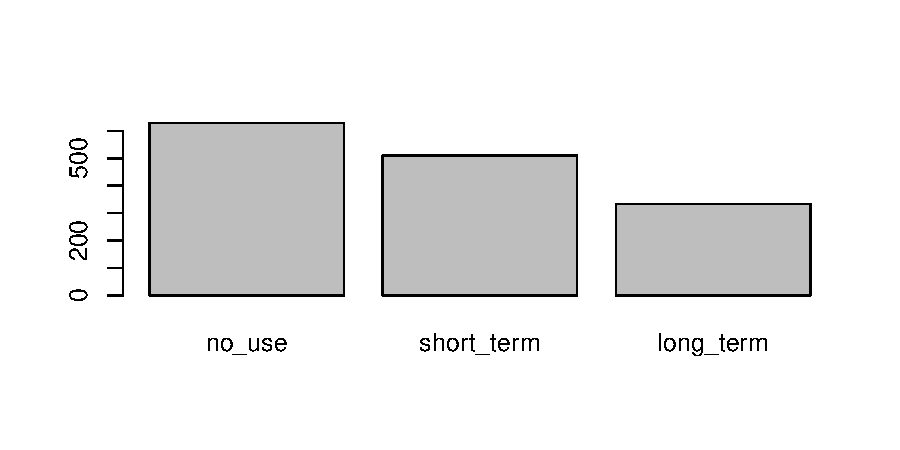
\includegraphics[width=\maxwidth]{figure/v:d:d-1} 

}



\end{knitrout}

\begin{enumerate}
\item[$1.1$] Es un multinomial ordenado. Corresponde o un ordered probit o un ordered logit.
\item[$1.2$] La diferencia es que en la especificaci\'on probit {\bf el error} est\'a distribuido normalmente (con promedio 0 y varianza 1), mientras que la distribucion logit {\bf el error} tiene un promedio 0 y una varianza $\frac{\pi^{2}}{3}$. {\bf El estudiante debe mencionar todo esto}.
\end{enumerate}


\section{2}

En este caso, estimaremos el modelo seg\'un las variables que se especifican. El estudiante puede hacer su propia selecci\'on de variables. {\bf Siempre deben estar justificadas}. Ambos modelos deben ser iguales en el n\'umero y tipo de variables independientes.

\begin{enumerate}
\item[$2.1$] Variables se muestran abajo. No incluyo justificaci\'on aqu\'i porque esto depender\'a de la selecci\'on del estudiante. Se incluye tabla.
\end{enumerate}

\begin{knitrout}
\definecolor{shadecolor}{rgb}{0.969, 0.969, 0.969}\color{fgcolor}\begin{kframe}
\begin{alltt}
\hlkwd{p_load}\hlstd{(MASS)}
\hlstd{o.logit} \hlkwb{=} \hlkwd{polr}\hlstd{(cmc} \hlopt{~} \hlstd{wife_edu} \hlopt{+} \hlstd{wife_age} \hlopt{+} \hlstd{num_child} \hlopt{+} \hlstd{islam} \hlopt{+} \hlstd{wife_working,}
\hlkwc{data} \hlstd{= dat,} \hlkwc{method} \hlstd{=} \hlstr{"logistic"}\hlstd{)}
\hlstd{o.probit} \hlkwb{=} \hlkwd{polr}\hlstd{(cmc} \hlopt{~} \hlstd{wife_edu} \hlopt{+} \hlstd{wife_age} \hlopt{+} \hlstd{num_child} \hlopt{+} \hlstd{islam} \hlopt{+} \hlstd{wife_working,}
\hlkwc{data} \hlstd{= dat,} \hlkwc{method} \hlstd{=} \hlstr{"probit"}\hlstd{)}
\end{alltt}
\end{kframe}
\end{knitrout}

Hagamos la tabla.

\begin{kframe}
\begin{alltt}
\hlkwd{p_load}\hlstd{(texreg)}
\hlkwd{texreg}\hlstd{(}\hlkwd{list}\hlstd{(o.logit, o.probit))} \hlcom{# usa "screenreg" no "texreg".}
\end{alltt}
\end{kframe}
\begin{table}
\begin{center}
\begin{tabular}{l c c}
\hline
 & Model 1 & Model 2 \\
\hline
wife\_edumid\_low      & $0.60^{**}$   & $0.36^{**}$   \\
                       & $(0.21)$      & $(0.12)$      \\
wife\_edumid\_high     & $1.11^{***}$  & $0.68^{***}$  \\
                       & $(0.21)$      & $(0.12)$      \\
wife\_eduhigh          & $1.99^{***}$  & $1.21^{***}$  \\
                       & $(0.21)$      & $(0.12)$      \\
wife\_age              & $-0.05^{***}$ & $-0.03^{***}$ \\
                       & $(0.01)$      & $(0.00)$      \\
num\_child             & $0.28^{***}$  & $0.16^{***}$  \\
                       & $(0.03)$      & $(0.02)$      \\
islam                  & $-0.46^{**}$  & $-0.27^{**}$  \\
                       & $(0.15)$      & $(0.09)$      \\
wife\_working          & $0.05$        & $0.03$        \\
                       & $(0.12)$      & $(0.07)$      \\
no\_use|short\_term    & $-0.13$       & $-0.03$       \\
                       & $(0.37)$      & $(0.22)$      \\
short\_term|long\_term & $1.58^{***}$  & $1.00^{***}$  \\
                       & $(0.37)$      & $(0.22)$      \\
\hline
AIC                    & $2925.06$     & $2924.57$     \\
BIC                    & $2972.71$     & $2972.23$     \\
Log Likelihood         & $-1453.53$    & $-1453.29$    \\
Deviance               & $2907.06$     & $2906.57$     \\
Num. obs.              & $1473$        & $1473$        \\
\hline
\multicolumn{3}{l}{\scriptsize{$^{***}p<0.001$; $^{**}p<0.01$; $^{*}p<0.05$}}
\end{tabular}
\caption{Statistical models}
\label{table:coefficients}
\end{center}
\end{table}



\begin{enumerate}
\item[$2.2$] Es esperable que el estudiante use el {\bf BIC} o {\bf AIC}. N\'umeros m\'as peque\~nos indican mejor \emph{fit}. En este caso, el modelo probit (``Model 2'') hace un mejor trabajo. Pero esto depender\'a de la selecci\'on de variables del estudiante. El estudiante tambi\'en puede usar el log-lik (numeros m\'as cercanos a cero son mejores).
\end{enumerate}

\section{3}

\begin{enumerate}
\item[$3$] El estudiante no necesariamente debe interpretar la tabla. Si lo hace, debe ser cap\'az de:
  \begin{enumerate}
    \item Decir ``cuando $x$ sube en una unidad, $y$ sube en $\beta$ ``log-odds'', manteniendo el resto de las variables constantes en su media.''
    \item El estudiante {\bf debe} identificar correctamente la unidad de cambio de los coeficientes: ``log-odds''.
  \end{enumerate}
\end{enumerate}

Calculemos ahora los \emph{predicted probabilities}. 

\begin{knitrout}
\definecolor{shadecolor}{rgb}{0.969, 0.969, 0.969}\color{fgcolor}\begin{kframe}
\begin{alltt}
\hlkwd{p_load}\hlstd{(effects)}
\hlkwd{plot}\hlstd{(}\hlkwd{effect}\hlstd{(}\hlstr{"wife_edu"}\hlstd{, o.logit))}
\end{alltt}
\end{kframe}

{\centering 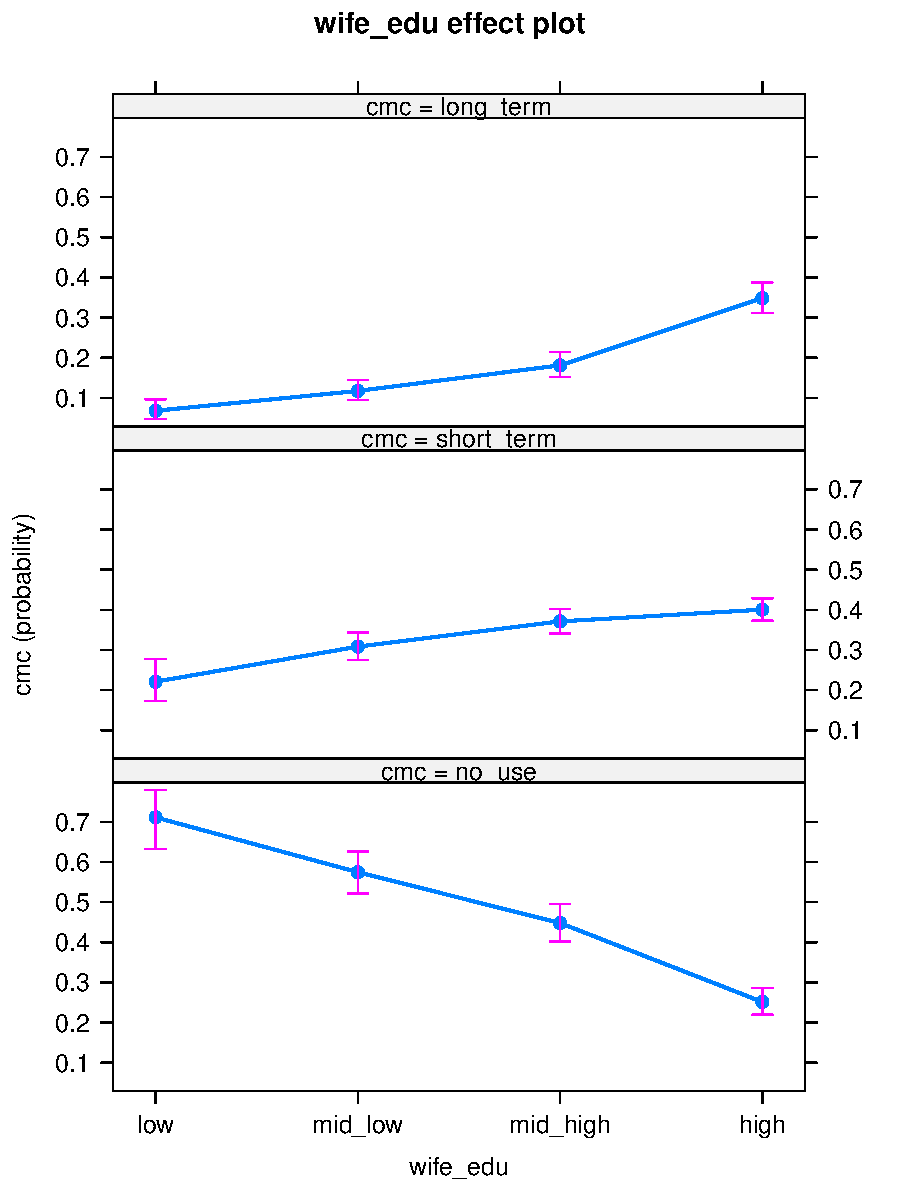
\includegraphics[width=\maxwidth]{figure/pp-1} 

}


\begin{kframe}\begin{alltt}
\hlkwd{plot}\hlstd{(}\hlkwd{effect}\hlstd{(}\hlstr{"wife_age"}\hlstd{, o.logit))}
\end{alltt}
\end{kframe}

{\centering 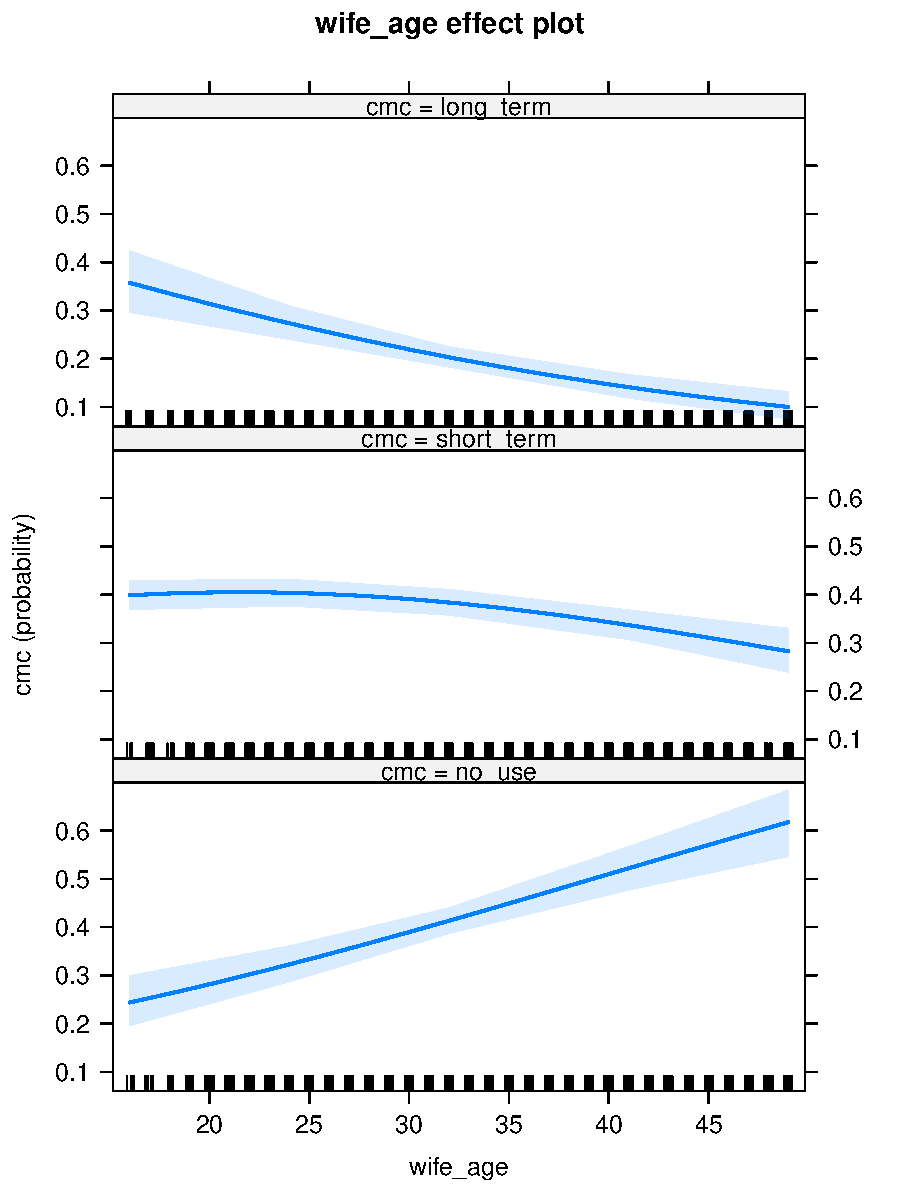
\includegraphics[width=\maxwidth]{figure/pp-2} 

}


\begin{kframe}\begin{alltt}
\hlkwd{plot}\hlstd{(}\hlkwd{effect}\hlstd{(}\hlstr{"num_child"}\hlstd{, o.logit))}
\end{alltt}
\end{kframe}

{\centering 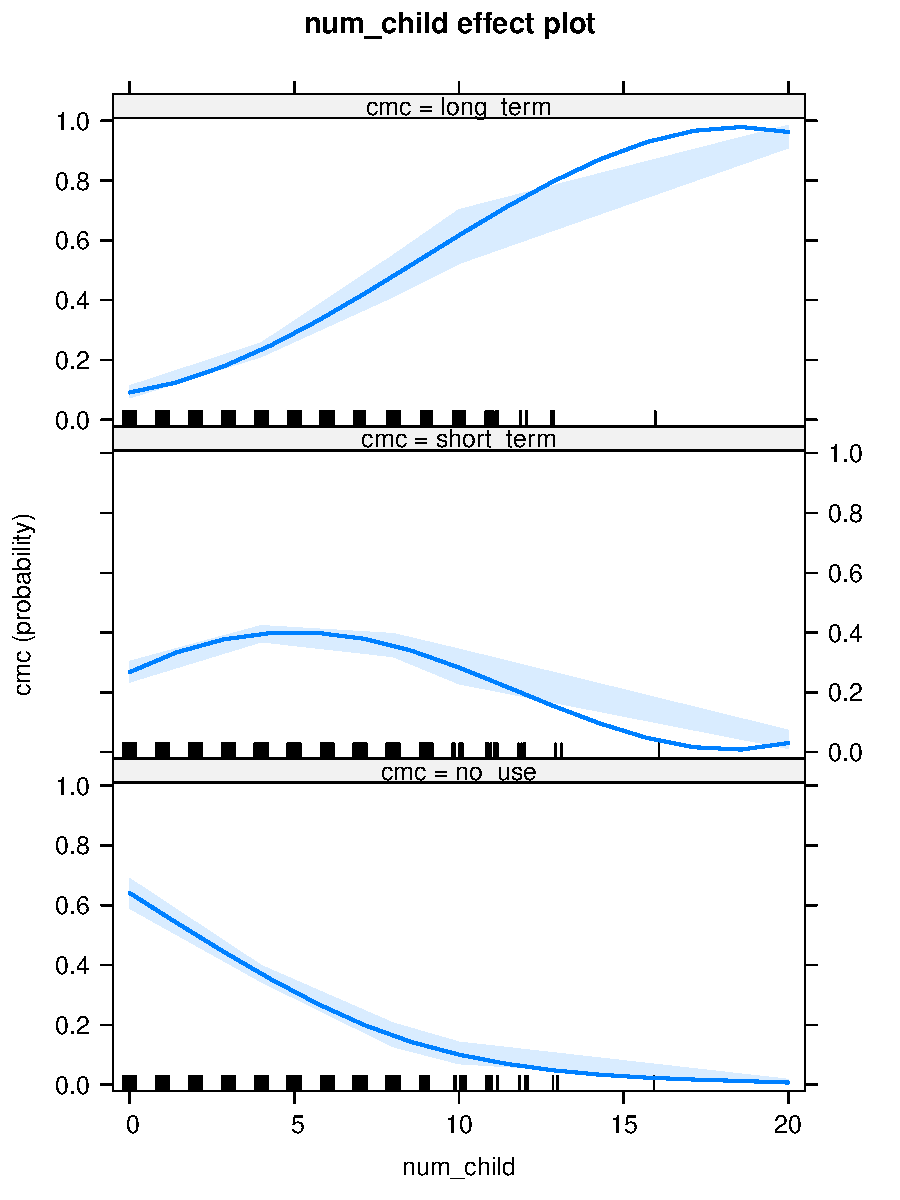
\includegraphics[width=\maxwidth]{figure/pp-3} 

}


\begin{kframe}\begin{alltt}
\hlkwd{plot}\hlstd{(}\hlkwd{effect}\hlstd{(}\hlstr{"islam"}\hlstd{, o.logit))}
\end{alltt}
\end{kframe}

{\centering 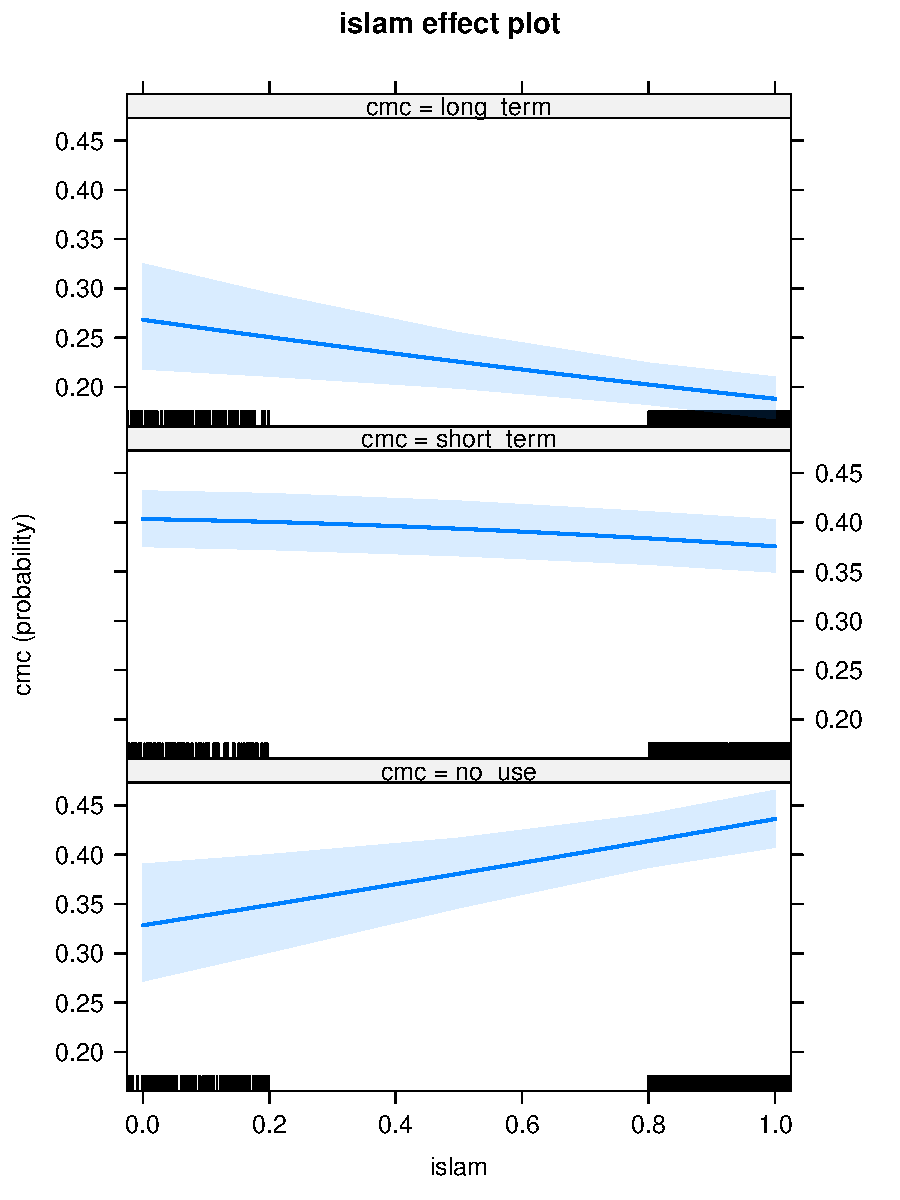
\includegraphics[width=\maxwidth]{figure/pp-4} 

}


\begin{kframe}\begin{alltt}
\hlkwd{plot}\hlstd{(}\hlkwd{effect}\hlstd{(}\hlstr{"wife_workin"}\hlstd{, o.logit))}
\end{alltt}


{\ttfamily\noindent\bfseries\color{errorcolor}{\#\# Error in Analyze.model(focal.predictors, mod, xlevels, default.levels, : the following predictor is not in the model: wife\_workin}}\end{kframe}
\end{knitrout}

No interpretar\'e las \emph{predicted probabilities} aqu\'i (ya que es contigente en el modelo del estudiante). El estudiante debe:

\begin{enumerate}
\item {\bf Interpretar \underline{todos} los par\'ametros de manera \underline{substantiva}}.
\item Seleccionar el set de interpretaciones en base al mejor modelo (en este caso, el modelo probit).
\item Identificar las unidades de los ejes de los gr\'aficos: el eje $Y$ es probabilidad, el eje $X$ son los niveles de las variables dependientes.
\end{enumerate}


%\newpage
%\paragraph{}
%\paragraph{}
%\pagenumbering{Roman}
%\setcounter{page}{1}
%\printbibliography



\end{document}


